\documentclass[11pt,a4paper,twocolumn]{IEEEtran}
\usepackage[utf8]{inputenc}
\usepackage{lipsum}
\usepackage{tabularx, booktabs}
\usepackage{amsmath}
\usepackage{amsfonts}
\usepackage{caption}
\usepackage{pdfpages}
\usepackage[margin=2.5cm]{geometry}
\usepackage{listings,lstautogobble}
\usepackage{amssymb}
\usepackage{hyperref}
\usepackage{graphicx}
\usepackage{svg}
\usepackage{pgf}
\usepackage{array}
\usepackage{cancel}
\usepackage{lipsum}
\usepackage{tikz}

\newcommand*\circled[2][1.6]{\tikz[baseline=(char.base)]{
		\node[shape=circle, draw, inner sep=1pt, 
		minimum height={\f@size*#1},] (char) {\vphantom{WAH1g}#2};}}
\newcommand{\sepline}{\noindent\makebox[\linewidth]{\rule{\textwidth}{1.2pt}}}
\newcommand{\bsepline}{\noindent\makebox[\linewidth]{\rule{7.5cm}{1.2pt}}}
\newcommand{\esepline}{\noindent\makebox[\linewidth]{\rule{7.5cm}{0.5pt}}}

\newcommand{\mysvg}[2]{\includesvg[width=0.#2\linewidth]{../svgs/#1}}
\newcommand*{\Scale}[2][4]{\scalebox{#1}{$#2$}}
\definecolor{RoyalBlue}{cmyk}{1, 0.50, 0, 0}
\lstset{language=Python,
	keywordstyle=\color{RoyalBlue},
	basicstyle=\fontsize{10}{10}\ttfamily,
	commentstyle=\ttfamily\itshape\color{gray},
	stringstyle=\ttfamily,
	showstringspaces=false,
	breaklines=true,
	frameround=ffff,
	rulecolor=\color{black},
	autogobble=true
}

\author{Saverio Monaco, Gerardo Carmona\\ 2012264\hspace{1.5cm} 2005005\\ \sepline}
\title{\textbf{Low Pass FIR Filter in FPGA}\\ Management and Analysis of Physics Datasets - MOD. A}


\begin{document}
	\maketitle
	\begin{abstract}
		FIR Filters are simple, yet effective filters which can be implemented in an FPGA. They may function as Low Pass, High Pass, Band Stop or Band Pass filters. We present a Low Pass FIR filter implementation which is connected to a UART source, fed by a simulated wave signal.
	\end{abstract}
	\section{FIR Filter}
	A Filter takes as input a signal $X[n]$ and outputs a refined one $Y[n]$. In the case of a FIR Filter, the law $X[n]\to Y[n]$ is described as follows: 
	$$ Y[n] = \sum_{i=0}^N C_i\, x[n-i] $$
	where $N$ is the \textit{filter order}. The filter performance improves as the order is increased. For this project, we have chosen to implement a 3 order filter (4-Taps FIR Filter).\\ Our transformation law is then
	$$\begin{aligned} Y[n]&=\sum_{i=0}^3 C_ix[n-i]=\\ & \Scale[0.8]{\hspace*{.2cm}=C_0x[n]+C_1x[n-1]+C_2x[n-2]+C_3x[n-3]}.\end{aligned}$$
	The filter described above has the following circuit representation:
	\begin{figure}[h]
		\centering
		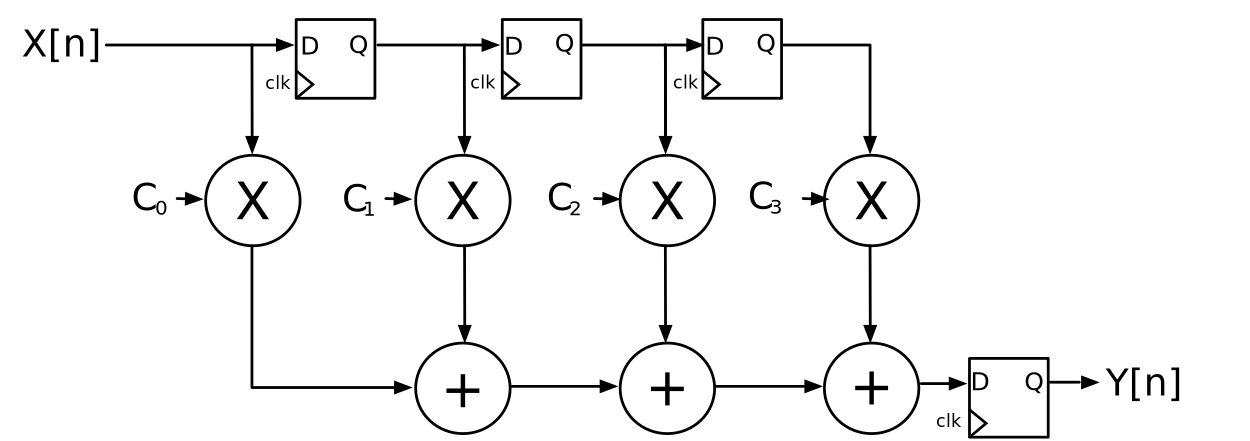
\includegraphics[width=1\linewidth]{img/FIR_direct_svg}
		\caption{Circuit for a FIR Filter}
	\end{figure}\\
	The square holds the place of a \emph{flip-flop} (necessary to store the past 3 inputs for the weighted sum), whereas the symbols 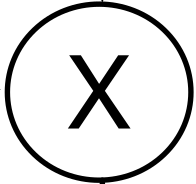
\includegraphics[width=0.05\linewidth]{img/x} and 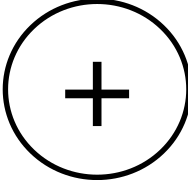
\includegraphics[width=0.05\linewidth]{img/+} correspond to the multiplication and addition operations, respectively.
	\subsection*{The coefficients}
	The value of the coefficients depends on the type of filter we wish to implement and the range of frequencies we aim to filter out.\\
	These values can be computed with the function \texttt{firwin} from the \emph{python} package \texttt{scipy}:
	\begin{lstlisting}
	from scipy import signal
	
	numtaps = 4
	f = 30
	
	signal.firwin(numtaps, f, fs=125)
	
	[0.0187 0.4812 0.4812 0.0187]
	\end{lstlisting}
	The coefficients so obtained will be used to build a low pass filter with a cut-off frequency of 30 Hz for a sampling frequency of 125 Hz
	\begin{figure}[h]
		\centering
		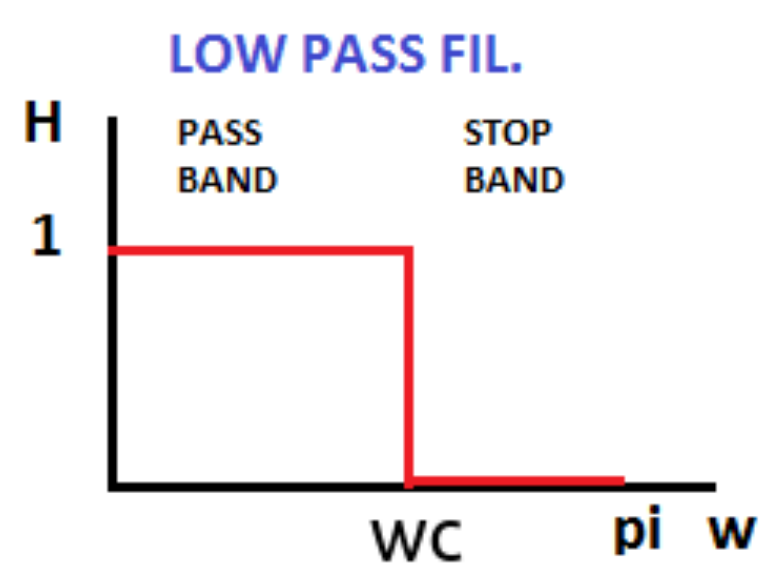
\includegraphics[width=0.7\linewidth]{img/lowpass}
		\caption{Low Pass filter}
	\end{figure}
	\section{Implementation of a FIR Filter in VHDL}
	Although these coefficients would ideally be implemented directly, the FPGA is unable to process floating point values. In order to overcome this, we proceed in the typical fashion of scaling the values and rounding them up once sufficient significant digits are guaranteed.\\
	For example:\\$$20\times 0.75 = 15$$ In binary this is translated to:
	$$ 10100_2 \times 0.11_2 = 1111_2.$$
	To realize this, we must scale the quantity $0.11_2$ through multiplication by $2^Q$ (resulting in a shift of bits) until we obtain an integer (or until we arbitrarly decide to truncate), then after the multiplication we can rescale back (shifting to the other direction):
	$$0.11_2 \times 2^3 = 0.11_2 <<3 = 110$$
	Now we can carry the multiplication
	$$10100_2\times 110_2 = 1111000_2,$$
	then we rescale back
	$$1111000_2 >> 3 = 1111_2 = 15.$$
	In practice, we scaled the coefficients and wrote them in hexadecimal:
	\begin{lstlisting}
	c = signal.firwin(4, 30, fs=125)
	rc = c * 2**8
	hex_rc = []
	
	for i in range(numtaps):
	hex_rc.append(hex(trunc_rc[i]))
	
	print(rc)    
	print(hex_rc)
	
	[0.0187 0.4812 0.4812 0.0187]
	['0x5', '0x7b', '0x7b', '0x5']
	\end{lstlisting}
	\subsection*{The algorithm}
	The product of an N-bits number and an M-bits one results in an (N+M)-bits number.\\
	When addition is performed, the number of bits in the result will be incremented by 1.\\
	Since the coefficients are 8 bits long, and the input signal is 8 bits long, the output signal should have 18 bits (see Fig. 3).\\
	In order to write a code able to compute this operation:
	$$ Y[n] = \sum_{i=0}^N C_i\, x[n-i] $$
	We implemented 5 processes in it:
	\begin{itemize}
	\item\textbf{p\_input} (initialization): The new value is stored in X[N] and the old ones are shifted one place to the right
	\item\textbf{p\_mult} (multiplication): Every value X[N-i] is multiplied by the coefficient $C_i$
	\item\textbf{p\_add\_0} (first additions): The additions $X[N]\times C_0 + X[N-1]\times C_1$ and $X[N-2]\times C_2 + X[N-3]\times C_3$ are performed and stored, with due care to avoid overflows
	\item\textbf{p\_add\_1} (final addition): The values of the last process are added together.
	\item\textbf{p\_output} (output): The 18 bits output is resized to 8 (same as the input)
	\end{itemize}
\begin{figure}[h]
	\hspace*{-.5cm}
	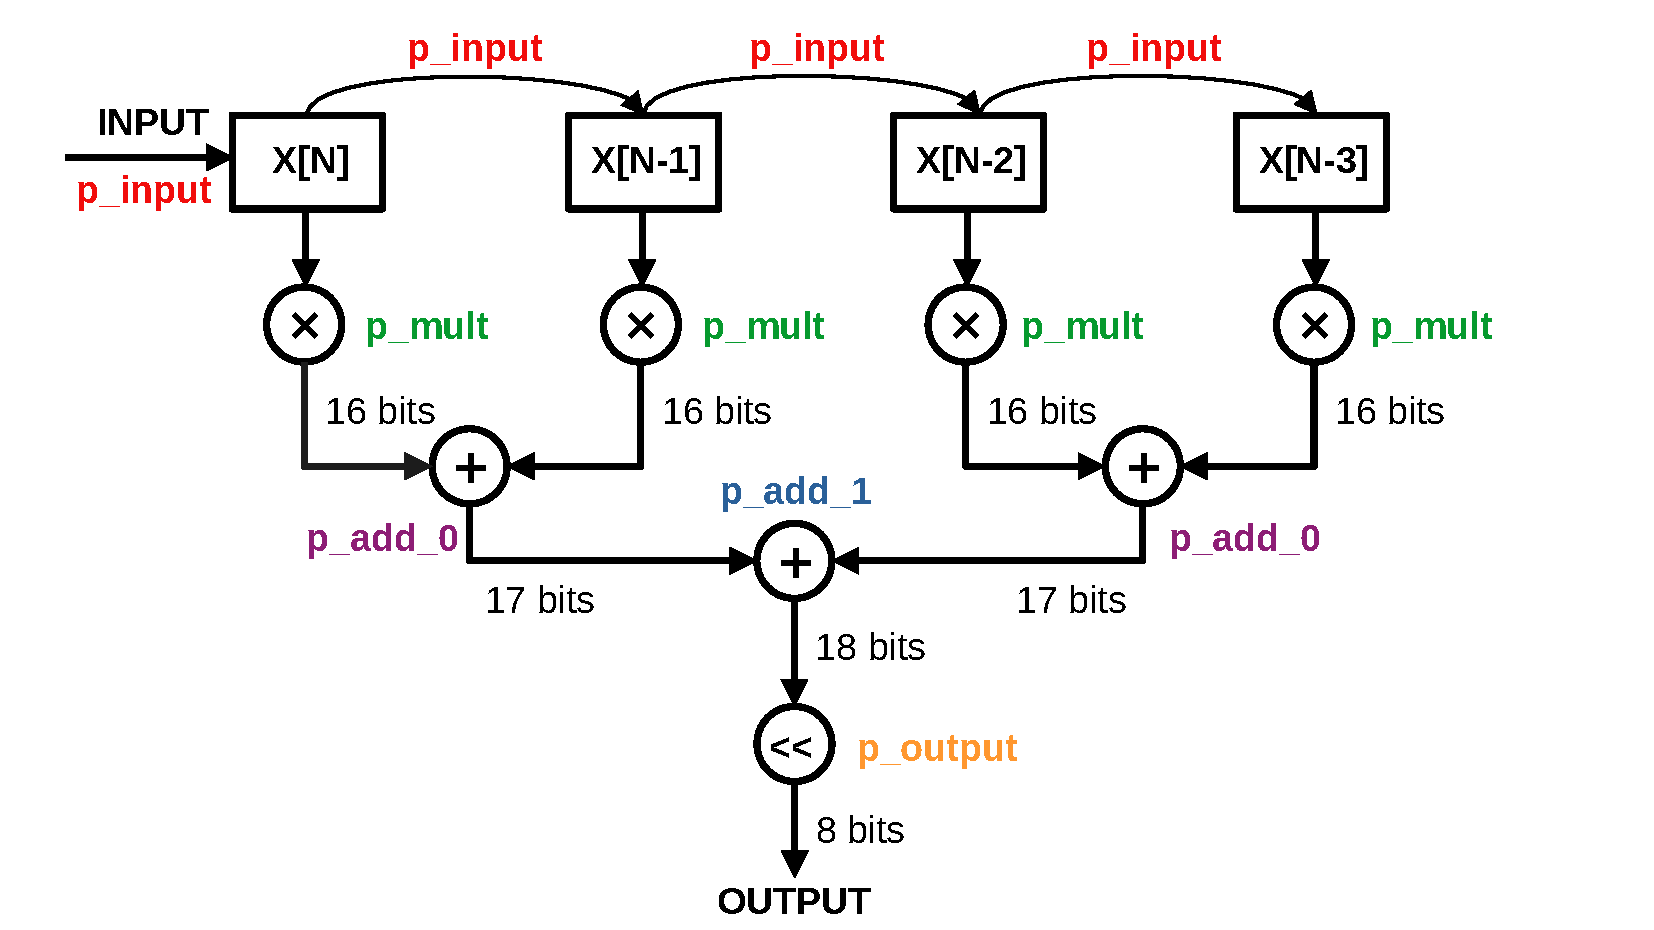
\includegraphics[width=1.2\linewidth]{img/firalg1pdf}
	\caption{Algorithm of FIR Filter}
\end{figure}
	\section{UART implementation}
	The UART is among the simplest devices capable of data exchange with the FPGA.
	To set up a UART correctly, the device and the FPGA must agree on how quickly the data is transfered, this speed is called \emph{Baud rate}.\\
	The data stream is the following:
	\begin{figure}[h]
		\centering
		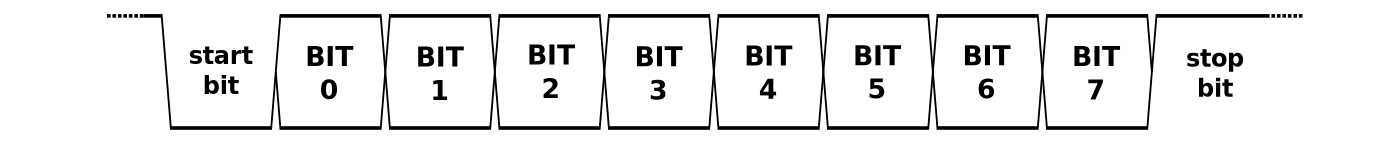
\includegraphics[width=1\linewidth]{img/UART_timing_diagram}
		\caption{UART communication}
	\end{figure}\\
	By default the \emph{Idle state} (in which the transmitter is waiting for data) is \texttt{HIGH}, the \emph{start bit} is \texttt{LOW}. No information is transfered with the start bit, it just states that data will  be transfered. Then the bits will be transfered, until the end of the stream is announced by the \emph{stop bit}, that is, a \texttt{HIGH} signal is received.\newpage
	The complete project can be schematized as it follows:
	\begin{figure}[h]
		\centering
		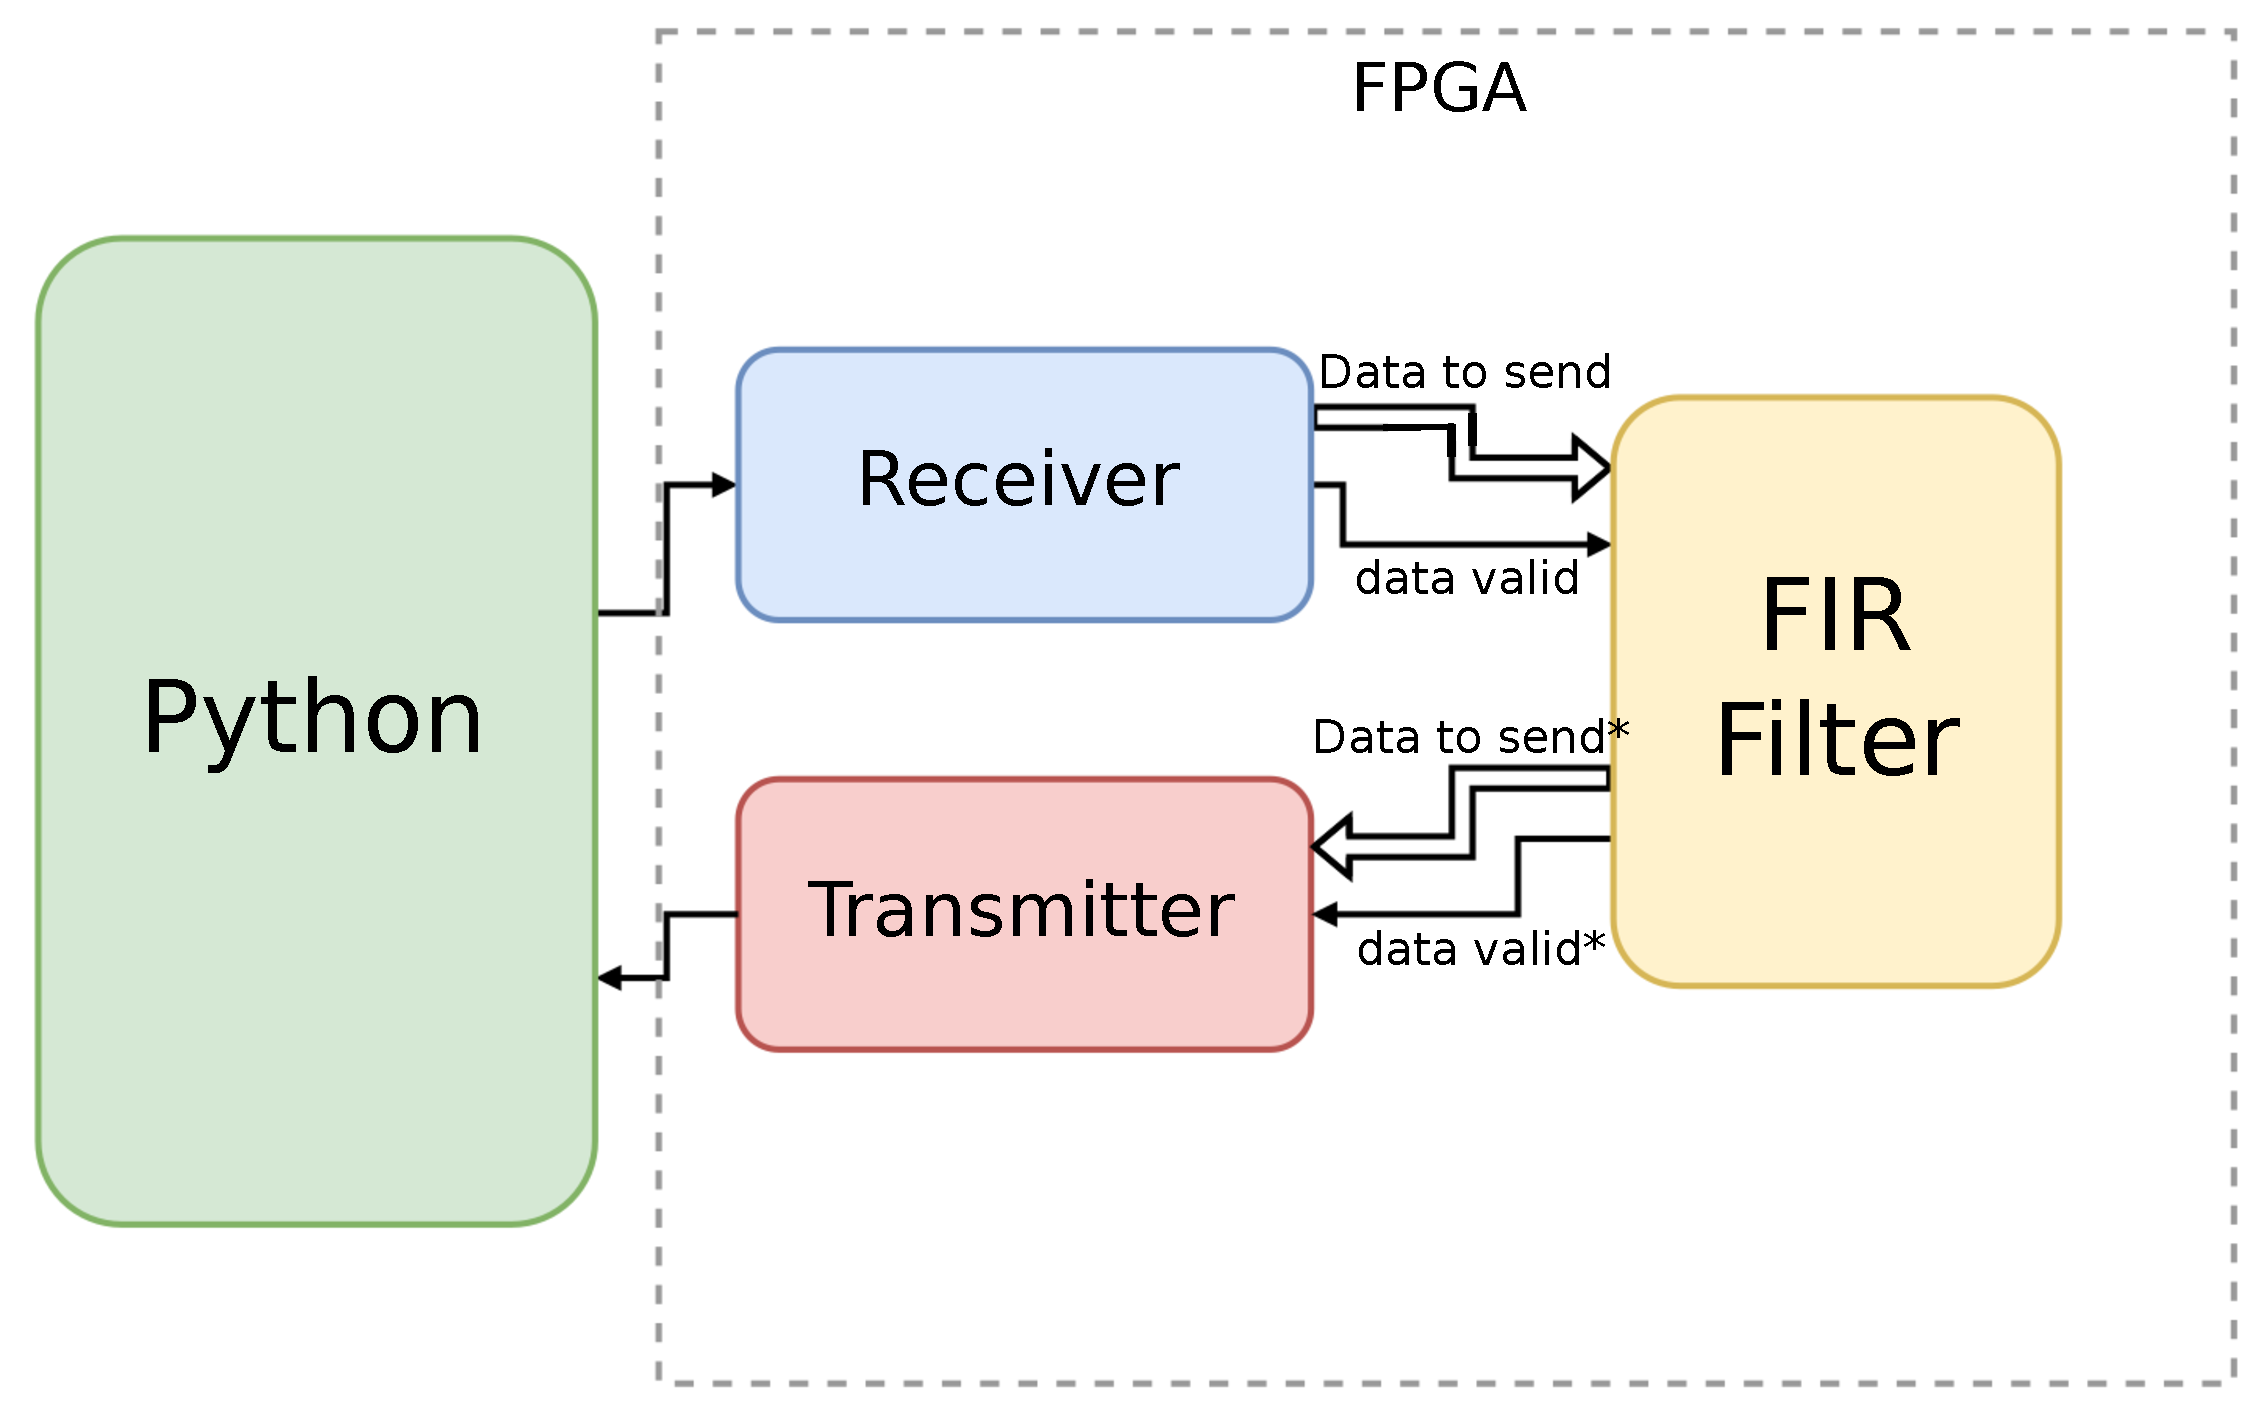
\includegraphics[width=1\linewidth]{img/projectcompletepdf}
		\caption{FPGA structure}
		\label{fig:fpgastruct}
	\end{figure}\\
	Inside the FPGA there is a \emph{receiver} that obtains data from a python script through a USB. The data is sent to the FIR Filter, where it is processed and then sent to the transmitter. Once there, the output can be read by python.\\
	For this project we need therefore three main entities: the FIR Filter, the Receiver and the Transmitter. All these entities are managed by another entity, named \emph{top}:
	\begin{figure}[h]
		\centering
		\vspace*{-.4cm}
		\hspace*{-.8cm}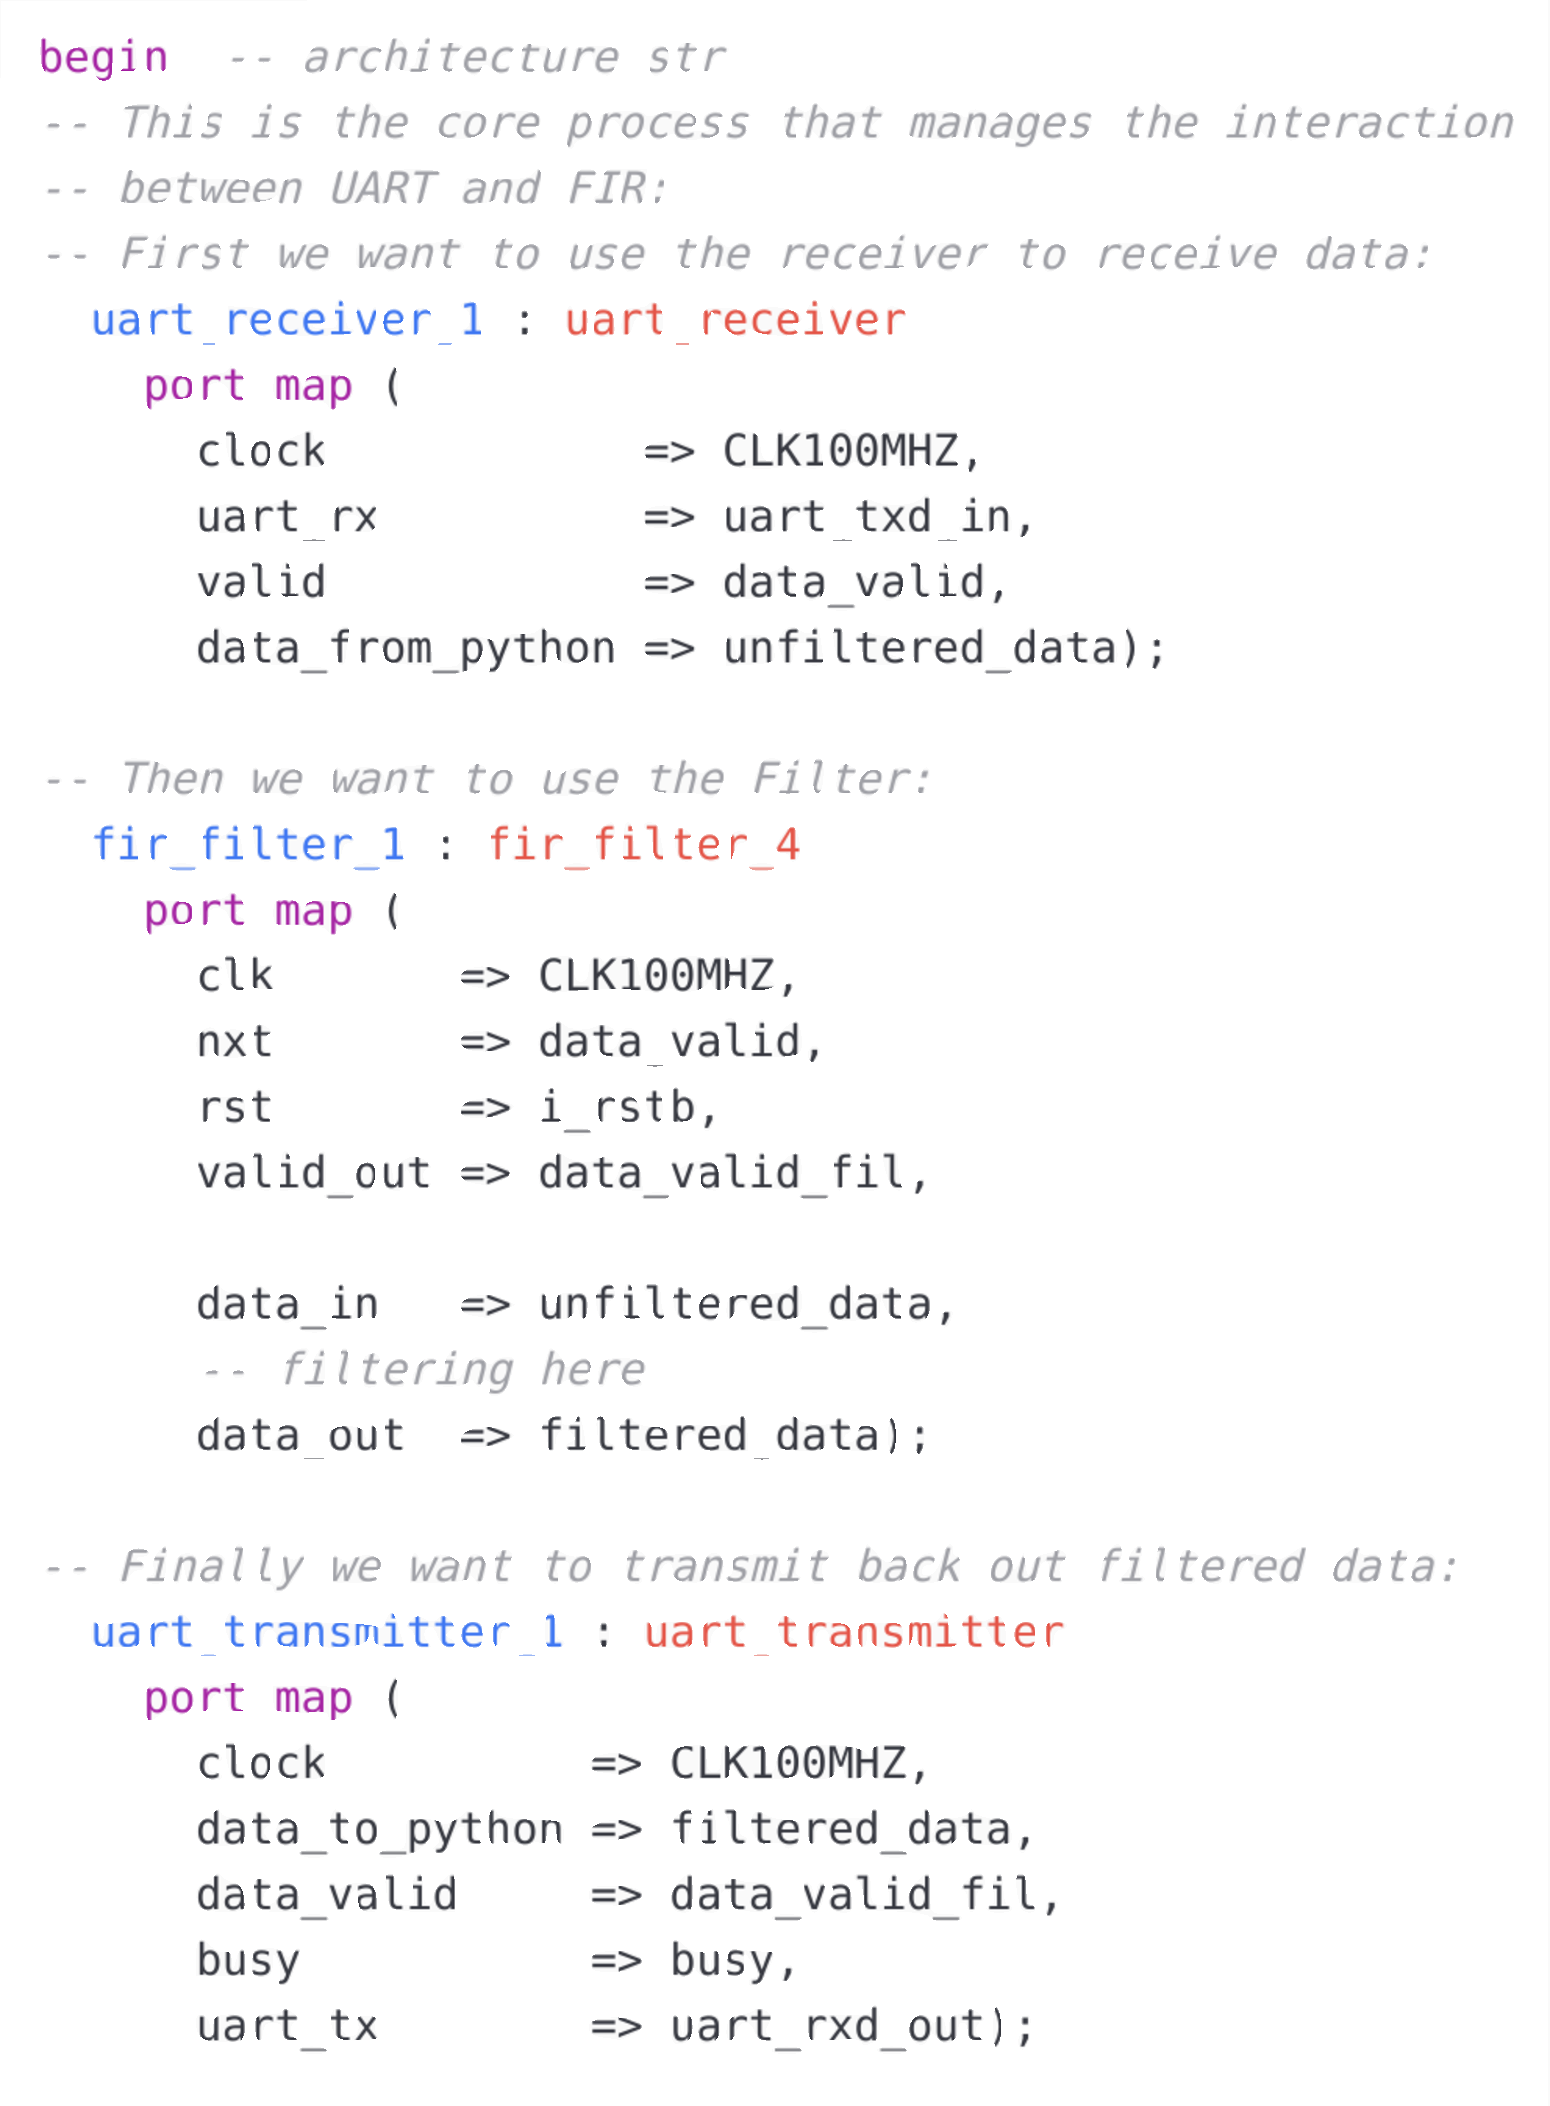
\includegraphics[width=1.2\linewidth]{img/code1white.png}
	\end{figure}
	\newpage
	\section{Results}
	The results shown correspond to an input signal of two frequencies, 10 Hz and 60 Hz: 
	\begin{figure}[h]
		\centering
		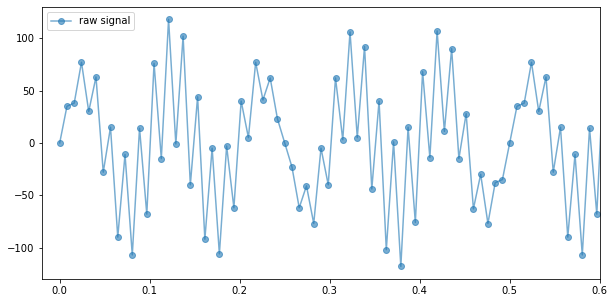
\includegraphics[width=.9\linewidth]{img/rawsig}
		\caption{Raw signal}
	\end{figure}\\
	Implementing a Filter with a cutoff frequency of 30 Hz, we get rid of the higher frequency (regarded as noise), obtaining the following result:
	\begin{figure}[h]
		\centering
		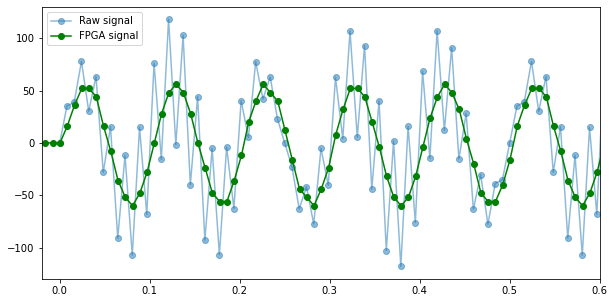
\includegraphics[width=.9\linewidth]{img/fpgaresult}
		\caption{FPGA performance}
	\end{figure}\\
	The output of the FPGA is a single frequency signal of 10 Hz, as expected. We can also compare the output from the FPGA and an FPGA simulation in Python using the function
	\begin{lstlisting}
	python_sig = lfilter(c, 1, wave)
	\end{lstlisting}
	Where \texttt{c} is the array of the coefficients and \texttt{wave} is the noisy signal input:
	\begin{figure}[h]
		\centering
		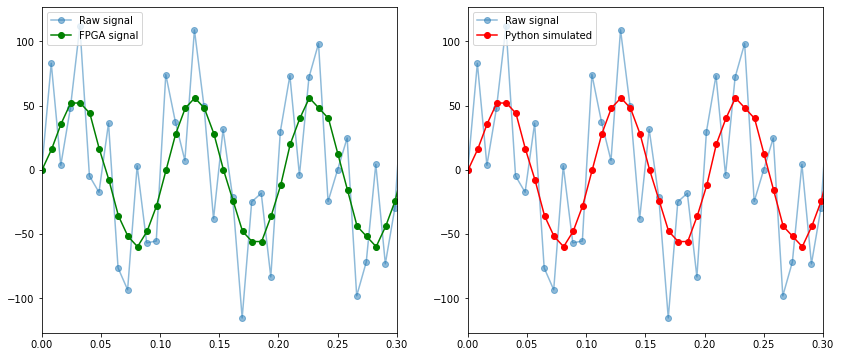
\includegraphics[width=1\linewidth]{img/fpgapython}
		\caption{Comparison with Python}
	\end{figure}\\
	\section{Conclusion}
	We implemented a four taps FIR filter, which successfully filtered the higher frequency signals from the simulated wave signal. We used a scaled, rounded-up value of the coefficients.
	Since results from the server FPGA optimally match the ones
	simulated in Python, we conclude that the FIR Filter has been properly implemented and that it
	efficiently simulates a low-pass filter.
\end{document}